%%%%%%%%%%%%%%%%%%%%
%%% Document
%%%%%%%%%%%%%%%%%%%%
\documentclass[pdftex, a4paper,11pt, twoside, ngerman]{report}
% \documentclass[11pt,xcolor=dvipsnames]{beamer}

% für deutsche zeichen äüö ohne kile auto-ersetzen
% \usepackage[utf8x]{inputenc}

% kile auto-ersetzen: einstellungen->latex:general-> hacken bei special
% characters
% \usepackage[ansinew]{inputenc}
% \usepackage[UKenglish]{babel}          %Englisch
\usepackage[ngerman]{babel}          %Deutsch


%%%%%%%%%%
%%% Geometry
%%%%%%%%%%
% \usepackage{showframe}
\usepackage[scale=0.8, hmarginratio=4:2]{geometry}
  \geometry{textheight=1.05\textheight, textwidth=.95\textwidth,
            marginparwidth=25 pt}
  \parskip=7pt

\renewcommand{\arraystretch}{1.2}

%%%%%%%%%%
%%% Packages (aus header datei)
%%%%%%%%%%
\IfFileExists{header_TobiasBrauell-DOCUMENT.tex}{
    % Copyright © 2014 Tobias Brauell <tobiasbrauell@gmail.com>

% This is my general purpose LaTeX header file for writing German documents.
% Ideally, you include this using a simple ``\input{header.tex}`` in your main
% document and start with ``\title`` and ``\begin{document}`` afterwards.

% If you need to add additional packages, I recommend not doing this in this
% file, but in your main document. That way, you can just drop in a new
% ``header.tex`` and get all the new commands without having to merge manually.

%%%%%%%%%%%%%%%%%%%%%%%%%%%%%
%%% Locale, date
%%%%%%%%%%%%%%%%%%%%%%%%%%%%%
\usepackage[UKenglish]{isodate}



%%%%%%%%%%%%%%%%%%%%%%%%%%%%%
%%% Margins and other spacing
%%%%%%%%%%%%%%%%%%%%%%%%%%%%%
\usepackage[activate]{pdfcprot}
% \usepackage[parfill]{parskip}
\usepackage{setspace}
  \setlength{\columnsep}{2 cm}
  \setlength{\parindent}{0 pt}


%%%%%%%%%%%%%%%%%%%%%%%%%%%%%
%%% Input encoding
%%%%%%%%%%%%%%%%%%%%%%%%%%%%%
\usepackage[T1]{fontenc}
\usepackage[utf8x]{inputenc}



%%%%%%%%%%%%%%%%%%%%%%%%%%%%%
%%% Indexing
%%%%%%%%%%%%%%%%%%%%%%%%%%%%%
\usepackage{makeidx}
  \makeindex



%%%%%%%%%%%%%%%%%%%%%%%%%%%%%
%%% Blindtext
%%%%%%%%%%%%%%%%%%%%%%%%%%%%%
\usepackage{blindtext}


%%%%%%%%%%%%%%%%%%%%%%%%%%%%%
%%% Global Counter
%%%%%%%%%%%%%%%%%%%%%%%%%%%%%



%%%%%%%%%%%%%%%%%%%%%%%%%%%%%
%%% Geometry
%%%%%%%%%%%%%%%%%%%%%%%%%%%%%
\usepackage{layout}
% \usepackage[scale=0.8]{geometry}
%   \geometry{textheight=1.05\textheight, marginparwidth=50 pt}

% \usepackage{multirow}
% \usepackage{dcolumn}



%%%%%%%%%%%%%%%%%%%%%%%%%%%%%
%%% Pagestyle
%%%%%%%%%%%%%%%%%%%%%%%%%%%%%
% \usepackage{fancyhdr}
% \usepackage{microtype} 

% \pagestyle{fancy}



%%%%%%%%%%%%%%%%%%%%%%%%%%%%%
%%% Fonts/Colors
%%%%%%%%%%%%%%%%%%%%%%%%%%%%%
\usepackage{lmodern}
\usepackage{xcolor}
% This replaces all fonts with Bitstream Charter, Bitstream Vera Sans and
% Bitstream Vera Mono. Math will be rendered in Charter.
% \usepackage[charter, greekuppercase=italicized]{mathdesign}
% \usepackage{beramono}
% \usepackage{berasans}

% Bold, sans-serif tensors. This fragment is taken from “egreg” from
% http://tex.stackexchange.com/a/82747/8945 and licensed under `CC-BY-SA
% <https://creativecommons.org/licenses/by-sa/3.0/>`_.
% \usepackage{bm}
%   \DeclareMathAlphabet{\mathsfit}{\encodingdefault}{\sfdefault}{m}{sl}
%   \SetMathAlphabet{\mathsfit}{bold}{\encodingdefault}{\sfdefault}{bx}{sl}
%   \newcommand{\tens}[1]{\bm{\mathsfit{#1}}}

% Bold vectors.
% \renewcommand{\vec}[1]{\boldsymbol{#1}}



%%%%%%%%%%%%%%%%%%%%%%%%%%%%%
%%% Code/Listings
%%%%%%%%%%%%%%%%%%%%%%%%%%%%%
\usepackage{listings}



%%%%%%%%%%%%%%%%%%%%%%%%%%%%%
%%% Enumerations
%%%%%%%%%%%%%%%%%%%%%%%%%%%%%
\usepackage{enumitem}
% \usepackage{paralist}


%%%%%%%%%%%%%%%%%%%%%%%%%%%%%
%%% Figures
%%%%%%%%%%%%%%%%%%%%%%%%%%%%%
% \usepackage[pdftex]{graphicx}
\usepackage{graphicx}
\usepackage{epsfig}
\usepackage{epstopdf}
\usepackage{subfigure}
\usepackage{wrapfig}
\makeatletter \newcommand\hyper@makecurrent[1]{} \makeatother
\usepackage{caption}
% \usepackage{subcaption}

\addto\captionsUKenglish{\renewcommand{\figurename}{Fig.}}
\addto\captionsngerman{\renewcommand{\figurename}{Abb.}}



%%%%%%%%%%%%%%%%%%%%%%%%%%%%%
%%% PDF Pages
%%%%%%%%%%%%%%%%%%%%%%%%%%%%%
\usepackage{pdfpages}



%%%%%%%%%%%%%%%%%%%%%%%%%%%%%
%%% Personal Graphics
%%%%%%%%%%%%%%%%%%%%%%%%%%%%%
\usepackage{tikz}
% \usepackage{tikz-3dplot}
  \usetikzlibrary{calc}
  \usetikzlibrary{decorations.markings}



%%%%%%%%%%%%%%%%%%%%%%%%%%%%%
%%% Math
%%%%%%%%%%%%%%%%%%%%%%%%%%%%%
\usepackage{amsmath}
\usepackage{amssymb}
\usepackage{mathtools}
\usepackage{dcolumn}
\usepackage{siunitx}
% \usepackage{feynmf}



%%%%%%%%%%%%%%%%%%%%%%%%%%%%%
%%% Referenzen
%%%%%%%%%%%%%%%%%%%%%%%%%%%%%
\usepackage{hyperref}
\usepackage{url}
% \usepackage{cleveref}%\label{abc}--\cref{abc} \Cref{abc[,def]}-und \crefrange{abc}{def}-bis
\usepackage[english]{cleveref}%\label{abc}--\cref{abc} \Cref{abc[,def]}-und \crefrange{abc}{def}-bis



%%%%%%%%%%%%%%%%%%%%%%%%%%%%%
%%% Table's
%%%%%%%%%%%%%%%%%%%%%%%%%%%%%
\usepackage{rotating}
\usepackage{longtable}
\usepackage{multirow}
\usepackage{tabularx}
  \newcolumntype{L}[1]{>{\raggedright\arraybackslash}p{#1}} % linksbündig mit Breitenangabe
  \newcolumntype{C}[1]{>{\centering\arraybackslash}p{#1}} % zentriert mit Breitenangabe
  \newcolumntype{R}[1]{>{\raggedleft\arraybackslash}p{#1}} % rechtsbündig mit Breitenangabe



%%%%%%%%%%%%%%%%%%%%%%%%%%%%%
%%% Todo's
%%%%%%%%%%%%%%%%%%%%%%%%%%%%%
% \usepackage{xkeyval}
\usepackage{todonotes} %\todo{text} oder \todo[inline]{text}
%   \presetkeys{todonotes}{inline}{}
%   \let\todox\todo
%   \renewcommand\todo{1}{\todox[inline]{#1}}


%%%%%%%%%%%%%%%%%%%%%%%%%%%%%%%%%%%%%%%%%%%%%%%%%%%%%%%%%%
%%% Settings
%%%%%%%%%%%%%%%%%%%%%%%%%%%%%%%%%%%%%%%%%%%%%%%%%%%%%%%%%%
\usepackage{cancel}

\newcommand{\HRule}{\rule{\linewidth}{0.5mm}}



%%%%%%%%%%%%%%%%%%%%%%%%%%%%%
%%% Theme
%%%%%%%%%%%%%%%%%%%%%%%%%%%%%



%%%%%%%%%%%%%%%%%%%%%%%%%%%%%
%%% header
%%%%%%%%%%%%%%%%%%%%%%%%%%%%%
% \lhead{text}
% \chead{text}
% \rhead{text}



%%%%%%%%%%%%%%%%%%%%%%%%%%%%%
%%% footer
%%%%%%%%%%%%%%%%%%%%%%%%%%%%%
%%% Tobias Brauell       	Versuch....		Ruth Jacobs
% \renewcommand\footrulewidth{.4pt}
% \lfoot{\scriptsize Ruth Jacobs - Tobias Brauell \\ {\ \ \ \ \ \ \ \ \ \ } Gruppe $\alpha 9$} 
% \cfoot{\thepage\ / \ \pageref{LastPage}}
% \rfoot{\scriptsize Versuch 518: Höhenstrahlung \\ Tutor: Christoph Krieger {\ \ \ } } 



%%%%%%%%%%%%%%%%%%%%%%%%%%%%%
%%% Title Page
%%%%%%%%%%%%%%%%%%%%%%%%%%%%%
% \title[ITER { } International Thermonuclear Experimental Reactor]{\huge{\bf{ITER}} \\ \large{\bf{International Thermonuclear Experimental Reactor}}}
% \author[T. Brauell]{Tobias Brauell}
% \institute{Universität Bonn}
% 
% \date{09.~Dez.~2013}
% \logo{\includegraphics[width=.15\textwidth]{Figures/toplogo.png}}


}{
    % Copyright © 2014 Tobias Brauell <tobiasbrauell@gmail.com>

% This is my general purpose LaTeX header file for writing German documents.
% Ideally, you include this using a simple ``\input{header.tex}`` in your main
% document and start with ``\title`` and ``\begin{document}`` afterwards.

% If you need to add additional packages, I recommend not doing this in this
% file, but in your main document. That way, you can just drop in a new
% ``header.tex`` and get all the new commands without having to merge manually.

%%%%%%%%%%%%%%%%%%%%%%%%%%%%%
%%% Locale, date
%%%%%%%%%%%%%%%%%%%%%%%%%%%%%
\usepackage[UKenglish]{isodate}



%%%%%%%%%%%%%%%%%%%%%%%%%%%%%
%%% Margins and other spacing
%%%%%%%%%%%%%%%%%%%%%%%%%%%%%
\usepackage[activate]{pdfcprot}
% \usepackage[parfill]{parskip}
\usepackage{setspace}
  \setlength{\columnsep}{2 cm}
  \setlength{\parindent}{0 pt}


%%%%%%%%%%%%%%%%%%%%%%%%%%%%%
%%% Input encoding
%%%%%%%%%%%%%%%%%%%%%%%%%%%%%
\usepackage[T1]{fontenc}
\usepackage[utf8x]{inputenc}



%%%%%%%%%%%%%%%%%%%%%%%%%%%%%
%%% Indexing
%%%%%%%%%%%%%%%%%%%%%%%%%%%%%
\usepackage{makeidx}
  \makeindex



%%%%%%%%%%%%%%%%%%%%%%%%%%%%%
%%% Blindtext
%%%%%%%%%%%%%%%%%%%%%%%%%%%%%
\usepackage{blindtext}


%%%%%%%%%%%%%%%%%%%%%%%%%%%%%
%%% Global Counter
%%%%%%%%%%%%%%%%%%%%%%%%%%%%%



%%%%%%%%%%%%%%%%%%%%%%%%%%%%%
%%% Geometry
%%%%%%%%%%%%%%%%%%%%%%%%%%%%%
\usepackage{layout}
% \usepackage[scale=0.8]{geometry}
%   \geometry{textheight=1.05\textheight, marginparwidth=50 pt}

% \usepackage{multirow}
% \usepackage{dcolumn}



%%%%%%%%%%%%%%%%%%%%%%%%%%%%%
%%% Pagestyle
%%%%%%%%%%%%%%%%%%%%%%%%%%%%%
% \usepackage{fancyhdr}
% \usepackage{microtype} 

% \pagestyle{fancy}



%%%%%%%%%%%%%%%%%%%%%%%%%%%%%
%%% Fonts/Colors
%%%%%%%%%%%%%%%%%%%%%%%%%%%%%
\usepackage{lmodern}
\usepackage{xcolor}
% This replaces all fonts with Bitstream Charter, Bitstream Vera Sans and
% Bitstream Vera Mono. Math will be rendered in Charter.
% \usepackage[charter, greekuppercase=italicized]{mathdesign}
% \usepackage{beramono}
% \usepackage{berasans}

% Bold, sans-serif tensors. This fragment is taken from “egreg” from
% http://tex.stackexchange.com/a/82747/8945 and licensed under `CC-BY-SA
% <https://creativecommons.org/licenses/by-sa/3.0/>`_.
% \usepackage{bm}
%   \DeclareMathAlphabet{\mathsfit}{\encodingdefault}{\sfdefault}{m}{sl}
%   \SetMathAlphabet{\mathsfit}{bold}{\encodingdefault}{\sfdefault}{bx}{sl}
%   \newcommand{\tens}[1]{\bm{\mathsfit{#1}}}

% Bold vectors.
% \renewcommand{\vec}[1]{\boldsymbol{#1}}



%%%%%%%%%%%%%%%%%%%%%%%%%%%%%
%%% Code/Listings
%%%%%%%%%%%%%%%%%%%%%%%%%%%%%
\usepackage{listings}



%%%%%%%%%%%%%%%%%%%%%%%%%%%%%
%%% Enumerations
%%%%%%%%%%%%%%%%%%%%%%%%%%%%%
\usepackage{enumitem}
% \usepackage{paralist}


%%%%%%%%%%%%%%%%%%%%%%%%%%%%%
%%% Figures
%%%%%%%%%%%%%%%%%%%%%%%%%%%%%
% \usepackage[pdftex]{graphicx}
\usepackage{graphicx}
\usepackage{epsfig}
\usepackage{epstopdf}
\usepackage{subfigure}
\usepackage{wrapfig}
\makeatletter \newcommand\hyper@makecurrent[1]{} \makeatother
\usepackage{caption}
% \usepackage{subcaption}

\addto\captionsUKenglish{\renewcommand{\figurename}{Fig.}}
\addto\captionsngerman{\renewcommand{\figurename}{Abb.}}



%%%%%%%%%%%%%%%%%%%%%%%%%%%%%
%%% PDF Pages
%%%%%%%%%%%%%%%%%%%%%%%%%%%%%
\usepackage{pdfpages}



%%%%%%%%%%%%%%%%%%%%%%%%%%%%%
%%% Personal Graphics
%%%%%%%%%%%%%%%%%%%%%%%%%%%%%
\usepackage{tikz}
% \usepackage{tikz-3dplot}
  \usetikzlibrary{calc}
  \usetikzlibrary{decorations.markings}



%%%%%%%%%%%%%%%%%%%%%%%%%%%%%
%%% Math
%%%%%%%%%%%%%%%%%%%%%%%%%%%%%
\usepackage{amsmath}
\usepackage{amssymb}
\usepackage{mathtools}
\usepackage{dcolumn}
\usepackage{siunitx}
% \usepackage{feynmf}



%%%%%%%%%%%%%%%%%%%%%%%%%%%%%
%%% Referenzen
%%%%%%%%%%%%%%%%%%%%%%%%%%%%%
\usepackage{hyperref}
\usepackage{url}
% \usepackage{cleveref}%\label{abc}--\cref{abc} \Cref{abc[,def]}-und \crefrange{abc}{def}-bis
\usepackage[english]{cleveref}%\label{abc}--\cref{abc} \Cref{abc[,def]}-und \crefrange{abc}{def}-bis



%%%%%%%%%%%%%%%%%%%%%%%%%%%%%
%%% Table's
%%%%%%%%%%%%%%%%%%%%%%%%%%%%%
\usepackage{rotating}
\usepackage{longtable}
\usepackage{multirow}
\usepackage{tabularx}
  \newcolumntype{L}[1]{>{\raggedright\arraybackslash}p{#1}} % linksbündig mit Breitenangabe
  \newcolumntype{C}[1]{>{\centering\arraybackslash}p{#1}} % zentriert mit Breitenangabe
  \newcolumntype{R}[1]{>{\raggedleft\arraybackslash}p{#1}} % rechtsbündig mit Breitenangabe



%%%%%%%%%%%%%%%%%%%%%%%%%%%%%
%%% Todo's
%%%%%%%%%%%%%%%%%%%%%%%%%%%%%
% \usepackage{xkeyval}
\usepackage{todonotes} %\todo{text} oder \todo[inline]{text}
%   \presetkeys{todonotes}{inline}{}
%   \let\todox\todo
%   \renewcommand\todo{1}{\todox[inline]{#1}}


%%%%%%%%%%%%%%%%%%%%%%%%%%%%%%%%%%%%%%%%%%%%%%%%%%%%%%%%%%
%%% Settings
%%%%%%%%%%%%%%%%%%%%%%%%%%%%%%%%%%%%%%%%%%%%%%%%%%%%%%%%%%
\usepackage{cancel}

\newcommand{\HRule}{\rule{\linewidth}{0.5mm}}



%%%%%%%%%%%%%%%%%%%%%%%%%%%%%
%%% Theme
%%%%%%%%%%%%%%%%%%%%%%%%%%%%%



%%%%%%%%%%%%%%%%%%%%%%%%%%%%%
%%% header
%%%%%%%%%%%%%%%%%%%%%%%%%%%%%
% \lhead{text}
% \chead{text}
% \rhead{text}



%%%%%%%%%%%%%%%%%%%%%%%%%%%%%
%%% footer
%%%%%%%%%%%%%%%%%%%%%%%%%%%%%
%%% Tobias Brauell       	Versuch....		Ruth Jacobs
% \renewcommand\footrulewidth{.4pt}
% \lfoot{\scriptsize Ruth Jacobs - Tobias Brauell \\ {\ \ \ \ \ \ \ \ \ \ } Gruppe $\alpha 9$} 
% \cfoot{\thepage\ / \ \pageref{LastPage}}
% \rfoot{\scriptsize Versuch 518: Höhenstrahlung \\ Tutor: Christoph Krieger {\ \ \ } } 



%%%%%%%%%%%%%%%%%%%%%%%%%%%%%
%%% Title Page
%%%%%%%%%%%%%%%%%%%%%%%%%%%%%
% \title[ITER { } International Thermonuclear Experimental Reactor]{\huge{\bf{ITER}} \\ \large{\bf{International Thermonuclear Experimental Reactor}}}
% \author[T. Brauell]{Tobias Brauell}
% \institute{Universität Bonn}
% 
% \date{09.~Dez.~2013}
% \logo{\includegraphics[width=.15\textwidth]{Figures/toplogo.png}}


}



%%%%%%%%%%
%%%%%%%%%%
%%%%%%%%%%
\begin{document}
%   \layout
  
  
  
  %%%%%%%%%%%%%%%%%%%%
  %%%%%%%%%%%%%%%%%%%%
  %%%%%%%%%%%%%%%%%%%%
  %%%%%%%%%%%%%%%%%%%%%%%%%%%%%%%%%%%%%%%%%%%%%%%%%%%%%%%%%%
%%% Title Page - Bachelor Thesis
%%%%%%%%%%%%%%%%%%%%%%%%%%%%%%%%%%%%%%%%%%%%%%%%%%%%%%%%%%
\begin{titlepage}
  \thispagestyle{empty}
  \begin{center}

    % Upper part of the page. The '~' is needed because \\
    % only works if a paragraph has started.
%     \includegraphics[width=0.15\textwidth]{./logo}~\\[1cm]
    \begin{minipage}{0.5\textwidth}
      \begin{flushleft}
	
\includegraphics[width=.5\textwidth]{Figures/logoUNI.png}
      \end{flushleft}
    \end{minipage}%
    \begin{minipage}{0.5\textwidth}
      \begin{flushright}
	
\includegraphics[width=.5\textwidth]{Figures/logoPI.png}
      \end{flushright}
    \end{minipage}
    
    \vspace{25 pt}
    
    \textsc{\LARGE Rheinische Friedrich-Wilhelms-Universität Bonn}\\[1.5 cm]
    
    \vspace{50 pt}
    
    \textsc{\Large Praktikum 4 - Atome und Moleküle}\\[0.5 cm]

    % Title
    \HRule \\[0.4 cm]
    { \huge \bfseries Versuch 424 - Hall-Effekt in Halbleitern \\[0.4 cm] }

    \HRule \\[1.5 cm]

    % Author and supervisor
    \noindent
    \begin{minipage}{0.4\textwidth}
      \begin{flushleft} \large
	\emph{Authors:}\\
	Tobias \textsc{Brauell}\\
	Frederike \textsc{Schrödel}
      \end{flushleft}
    \end{minipage}%
    \begin{minipage}{0.4\textwidth}
      \begin{flushright} \large
	\emph{Supervisor:} \\
	Farah Noreen \textsc{Afzal}
      \end{flushright}
    \end{minipage}

    \vfill

    % Bottom of the page
    \HRule \\[0.4 cm]
    {\large \today}

  \end{center}
\end{titlepage}
  %%%%%%%%%%%%%%%%%%%%
  
  
  
%   \setcounter{page}{2}
  
  \begin{chapter}*{Abstract}
    Ziel des Versuchs ist es...
    
    \todo{TO-DO}
    
  \end{chapter}
  
  \tableofcontents
  
  
  
  %%%%%%%%%%%%%%%%%%%%
  %%%%%%%%%%%%%%%%%%%%
  %%%%%%%%%%%%%%%%%%%%
  \begin{chapter}{Theorie des Versuchs}
    \label{chp:Theorie}
    
    
    
  \end{chapter}
  %%%%%%%%%%%%%%%%%%%%
         
         
         
  %%%%%%%%%%%%%%%%%%%%
  %%%%%%%%%%%%%%%%%%%%
  %%%%%%%%%%%%%%%%%%%%
  \begin{chapter}{Aufbau des Versuches}
    \label{chp:Aufbau}
    Der Aufbau dieses Versuches ist in \cref{fig:Aufbau} zu sehen.
    Die Probe wird im Rezipienten montiert und angeschlossen.
    An der Probe kann von außen ein Magnetfeld mittels eines permanent Magneten
    angelegt werden. An der Stromquelle wird ein Strom nach den Vorgaben der
    ausliegenden Anleitungen und der Art der Probe eingestellt.
    Dieser Strom bleibt für alle Messungen dieser Probe unbedingt konstant.
    An einem Voltmeter keine die anliegende Spannung gemessen werden.
    Stromquelle und Voltmeter sind über einen Schaltkasten mit der Probe im
    Rezipienten verbunden.
    Über den Schaltkasten lässt sich die Beschaltung der Probe mit zwei
    Drehreglern einstellen.
    Welche Art der Beschaltung zur Verfügung stehen kann ebenfalls in den
    ausliegenden Tabellen nachgeschlagen werden.
    Am benutzte permanent Magnet wurden die Pole markiert und kann um die Probe
    gedreht werden um die Ausrichtung des Magnetfeldes umzukehren.
    
    Weiter ist für den zweiten Teil dieses Versuches ein Helium Kühlaggregat am
    Rezipienten und eine Heizung am Probenträger selbst angebracht.
    Über das Kühlaggregat kann die Probe auf sehr niedrige Temperaturen
    abgekühlt werden. Zum erwärmen, kann ein Strom von einer zweiten Stromquelle
    durch den Heizdraht geschickt werden. Die Temperatur der Probe kann über
    die Spannung an einem Temperatursensor und einer ausliegenden
    Tabelle umgerechnet werden.
    Für die Messung der Temperaturabhängigkeit wird der Rezipient auf einen
    Druck von etwa \SI{1e-8}{\bar} evakuiert.
    
    \todo{Graphischen Aufbau machen!}
    
  \end{chapter}
  %%%%%%%%%%%%%%%%%%%%
  
  
  
  %%%%%%%%%%%%%%%%%%%%
  %%%%%%%%%%%%%%%%%%%%
  %%%%%%%%%%%%%%%%%%%%
  \begin{chapter}{Durchführung der Messungen}
    \label{chp:Durchführung}
    
    
    
    %%%%%%%%%%%%%%%%%%%%%%%%%%%%%%
    %%%%%%%%%%%%%%%%%%%%%%%%%%%%%%
    %%%%%%%%%%%%%%%%%%%%%%%%%%%%%%
    \begin{section}{Messung des Widerstandes bei Raumtemperatur}
      \label{chp:MessungWiderstandRaumtemperatur}
      Die Messung des Widerstandes führen wir für die Proben
      \textit{GaAs (alt)} bei \SI{100,000(5)}{\micro\ampere} und
      \textit{InAs - HF-301-040} bei \SI{15,003(5)}{\milli\ampere} durch.
      Die Raumtemperatur bei den Messungen betrug \SI{26}{\celsius} und die
      stärke des permanent Magneten ist mit \SI{0,138(1)}{\tesla} angegeben.
      \begin{table}[hb]
        \centering
        \footnotesize
        \rowcolors{2}{}{lightgray!40}
        \begin{tabular}{cccccccc}
          Schaltung & $U / mV$  & $U / mV$  & $U / mV$  & $U / mV$  & $U / mV$
               & $<U> / mV$  & $\sigma(<U>) / mV$ \\ \hline \hline
          % & mess & nr. & durchgang & 1 & durchgang & 2 & durchgang & 3 & durchgang & 4 & durchgang & 5 & Average & std & dev \\ 
1 & -0,244 & -0,244 & -0,244 & -0,244 & -0,243 & -0,2438 & 0,0004 \\ 
2 & 0,241 & 0,241 & 0,242 & 0,242 & 0,241 & 0,2414 & 0,000489898 \\ 
3 & -0,193 & -0,193 & -0,193 & -0,193 & -0,193 & -0,193 & 0 \\ 
4 & 0,19 & 0,19 & 0,19 & 0,19 & 0,19 & 0,19 & 0 \\ 
5 & -0,243 & -0,243 & -0,243 & -0,243 & -0,242 & -0,2428 & 0,0004 \\ 
6 & 0,242 & 0,242 & 0,242 & 0,242 & 0,242 & 0,242 & 0 \\ 
7 & -0,193 & -0,192 & -0,193 & -0,192 & -0,192 & -0,1924 & 0,000489898 \\ 
8 & 0,19 & 0,191 & 0,19 & 0,19 & 0,191 & 0,1904 & 0,000489898 \\ 

        \end{tabular}
        \caption{Messdaten der Widerstands Messung für die \textit{GaAs (alt)}
            Probe.}
        \label{tab:WiderstandGaAs}
      \end{table}
      \begin{table}[hb]
        \centering
        \footnotesize
        \rowcolors{2}{}{lightgray!40}
        \begin{tabular}{cccccccc}
          Schaltung & $U / mV$  & $U / mV$  & $U / mV$  & $U / mV$  & $U / mV$
               & $<U> / mV$  & $\sigma(<U>) / mV$ \\ \hline \hline
          % & Mess & Nr & Spannung & 1 & Spannung & 2 & Spannung & 3 & Spannung & 4 & Spannung & 5 & average \\ \hline
1 & -89,887 & -89,905 & -89,907 & -89,905 & -89,91 & -89,9028 & 0,008109254 \\ \hline
2 & 89,848 & 89,864 & 89,866 & 89,866 & 89,868 & 89,8624 & 0,007310267 \\ \hline
3 & -89,529 & -89,543 & -89,544 & -89,545 & -89,546 & -89,5414 & 0,006280127 \\ \hline
4 & 89,484 & 89,497 & 89,499 & 89,5 & 89,501 & 89,4962 & 0,006241795 \\ \hline
5 & -89,848 & -89,86 & -89,861 & -89,863 & -89,864 & -89,8592 & 0,005775812 \\ \hline
6 & 89,889 & 89,898 & 89,9 & 89,902 & 89,904 & 89,8986 & 0,0052 \\ \hline
7 & -89,492 & -89,5 & -89,501 & -89,503 & -89,505 & -89,5002 & 0,004445222 \\ \hline
8 & 89,538 & 89,546 & 89,549 & 89,55 & 89,551 & 89,5468 & 0,004707441 \\ \hline

        \end{tabular}
        \caption{Messdaten der Widerstands Messung für die
            \textit{InAs - HF-301-040} Probe.}
        \label{tab:WiderstandInAs}
      \end{table}
      Für beide Proben messen wir die Spannungen aller acht Schaltungen zur
      Bestimmung des Widerstandes. Um die Messwerte statistisch mitteln zu
      können, nehmen wir für jede Schaltung fünf verschiedene Werte.
      Hierbei ist $<U>$ der statistische Mittelwert und $\sigma(<U>)$ die
      Standardabweichung des Mittelwertes.
      Die gewonnenen Messwerte können in
      \cref{tab:WiderstandGaAs,tab:WiderstandInAs} eingesehen werden.
      
      
    \end{section}
    %%%%%%%%%%%%%%%%%%%%%%%%%%%%%%
    
    
    
    %%%%%%%%%%%%%%%%%%%%%%%%%%%%%%
    %%%%%%%%%%%%%%%%%%%%%%%%%%%%%%
    %%%%%%%%%%%%%%%%%%%%%%%%%%%%%%
    \begin{section}{Messung der Hallkonstanten bei Raumtemperatur}
      \label{chp:MessungHallkonstanteRaumtemperatur}
      Bei der Messung der Hallkonstanten bei Raumtemperatur wird dem Aufbau der
      permanent Magnet hinzugefügt und die Schaltungen zur Messung der
      Hallkonstanten verwendet.
      Auch hier nehmen wir wieder fünf Werte und bilden den Mittelwert um
      statistisch aussagekräftige Messwerte und statistische Fehler zu erhalten.
      Hierbei ist $<U>$ wieder der statistische Mittelwert und $\sigma(<U>)$ die
      Standardabweichung des Mittelwertes.
      Die gewonnenen Messwerte können in
      \cref{tab:HallGaAs,tab:HallInAs} eingesehen werden.
      \begin{table}[htbp]
        \centering
        \footnotesize
        \rowcolors{2}{}{lightgray!40}
        \begin{tabular}{ccccccccc}
          Schaltung & Magn. & $U / mV$ & $U / mV$  & $U / mV$  & $U / mV$  & $U / mV$
               & $<U> / mV$  & $\sigma(<U>) / mV$ \\ \hline \hline
          % & mess & nr \\ \hline
1 & $B+$ & -0,008 & -0,008 & -0,008 & -0,007 & -0,007 & -0,0076 & 0,000489898 \\ 
2 & $B+$ & 0,005 & 0,006 & 0,006 & 0,006 & 0,006 & 0,0058 & 0,0004 \\
3 & $B+$ & 0,094 & 0,094 & 0,094 & 0,095 & 0,095 & 0,0944 & 0,000489898 \\ 
4 & $B+$ & -0,097 & -0,096 & -0,0965 & -0,096 & -0,096 & -0,0963 & 0,0004 \\ 
5 & $B-$ & -0,096 & -0,097 & -0,096 & -0,096 & -0,095 & -0,096 & 0,000632456 \\ 
6 & $B-$ & 0,056 & 0,095 & 0,095 & 0,096 & 0,095 & 0,0874 & 0,015704776 \\ 
7 & $B-$ & 0,005 & 0,005 & 0,005 & 0,005 & 0,006 & 0,0052 & 0,0004 \\ 
8 & $B-$ & -0,008 & -0,008 & -0,008 & -0,008 & -0,007 & -0,0078 & 0,0004 \\ 
9 & 0 & -0,051 & -0,051 & -0,051 & -0,051 & -0,05 & -0,0508 & 0,0004 \\ 
10 & 0 & 0,05 & 0,05 & 0,05 & 0,05 & 0,051 & 0,0502 & 0,0004 \\ 

        \end{tabular}
        \caption{Messdaten zur Bestimmung der Hallkonstanten für die
            \textit{GaAs (alt)} Probe.}
        \label{tab:HallGaAs}
      \end{table}
      \begin{table}[htbp]
        \centering
        \footnotesize
        \rowcolors{2}{}{lightgray!40}
        \begin{tabular}{ccccccccc}
          Schaltung & Magn. & $U / mV$ & $U / mV$  & $U / mV$  & $U / mV$  & $U / mV$
               & $<U> / mV$  & $\sigma(<U>) / mV$ \\ \hline \hline
          % & Mess & Nr & Spannung & 1 & Spannung & 2 & Spannung & 3 & Spannung & 4 & Spannung & 5 \\ 
1 & $B+$ & 26,524 & 26,516 & 26,516 & 26,513 & 26,499 & 26,5136 & 0,008163333 \\ 
2 & $B+$ & -26,462 & -26,454 & -26,454 & -26,451 & -26,437 & -26,4516 & 0,008163333 \\ 
3 & $B+$ & 27,192 & 27,184 & 27,184 & 27,182 & 27,169 & 27,1822 & 0,00744043 \\ 
4 & $B+$ & -27,203 & -27,194 & -27,194 & -27,192 & -27,178 & -27,1922 & 0,008059777 \\ 
5 & $B-$ & -27,196 & -27,199 & -27,193 & -27,187 & -27,18 & -27,191 & 0,00678233 \\ 
6 & $B-$ & 27,26 & 27,263 & 27,257 & 27,25 & 27,243 & 27,2546 & 0,007227724 \\ 
7 & $B-$ & -26,501 & -26,504 & -26,496 & -26,49 & -26,484 & -26,495 & 0,007266361 \\ 
8 & $B-$ & 26,495 & 26,499 & 26,492 & 26,486 & 26,479 & 26,4902 & 0,007025667 \\ 
9 & 0 & -0,33 & -0,33 & -0,331 & -0,329 & -0,331 & -0,3302 & 0,000748331 \\ 
10 & 0 & 0,394 & 0,393 & 0,393 & 0,394 & 0,393 & 0,3934 & 0,000489898 \\ 

        \end{tabular}
        \caption{Messdaten zur Bestimmung der Hallkonstanten für die
            \textit{InAs - HF-301-040} Probe.}
        \label{tab:HallInAs}
      \end{table}
      
      Bei den Schaltungen $1-4$ wird das externe Magnetfeld in \textit{$B+$}
      angelegt, d.h. der markierte Nordpol des permanent Magneten liegt auf
      der Seite des Probenträger, auf dem die Probe montiert ist.
      Schaltungen $5-8$ wird in \textit{$B-$} gemessen. Dabei wird der Magnet
      kurzerhand um \SI{180}{\degree} gedreht, sodass nun der Südpol zur Probe
      zeigt.
      Die Schaltungen $9-10$ werden ohne den externen Magneten gemessen.
      
      
    \end{section}
    %%%%%%%%%%%%%%%%%%%%%%%%%%%%%%
    
    
    
    %%%%%%%%%%%%%%%%%%%%%%%%%%%%%%
    %%%%%%%%%%%%%%%%%%%%%%%%%%%%%%
    %%%%%%%%%%%%%%%%%%%%%%%%%%%%%%
    \begin{section}{Messungen bei unterschiedlichen Temperaturen}
      \label{chp:MessungUnterschiedlicheTemperaturen}
      Nachdem alle Messungen am ersten Tag abgeschlossen sind schalten wir die
      Vakuum Turbopumpe und die Helium Kühlung des Rezipienten ein.
      Dabei haben wir die Probe \textit{InAs - HF-301-040} für die kommenden
      Messungen im Rezipienten.
      An dem angeschlossenen Voltmeter lässt sich die Thermospannung ablesen
      und mit der ausliegenden Tabelle in \SI{}{\celsius} umrechnen.
      Über Nacht wurde die Probe auf etwa \SI{-205}{\kelvin} abgekühlt.
      Nun messen wir die Temperaturabhängigkeiten des Widerstandes und der
      Hallkonstante. Dazu messen wir alle $18$ Schaltungen bei einer Temperatur
      jeweils einmal, sobald wir mithilfe der Heizung die Temperatur
      stabilisiert haben.
      
      \todo{noch was zur Durchführung?}
      
      In \cref{tab:TemperaturInAs} sind alle Messwerte
      festgehalten. Die Temperatur wurde während der Messung direkt von
      uns gegen die Raumtemperatur korrigiert.
      \begin{sidewaystable}[htbp]
        \centering
        \footnotesize
        \rowcolors{3}{}{lightgray!40}
        \begin{tabular}{c c c c c c c c c c c c c c c}
          % \cline{2-15}
\\ \hline
\hiderowcolors 
\multicolumn{15}{|c|}{Temperaturen der Messungen $/K$} \\ \hline
Messung: & 1 & 2 & 3 & 4 & 5 & 6 & 7 & 8 & 9 & 10 & 11 & 12 & 13 & 14 \\
\showrowcolors
$t_1$ & -206 & -196 & -183 & -172 & -163 & -153 & -140 & -125 & -110 & -93 & -79 & -64 & -27 & 0 \\
$t_2$ & -205 & -195 & -183 & -173 & -160 & -151 & -140 & -125 & -109 & -93 & -79 & -62 & -27 & 0 \\
$<t>$ & -205,5 & -195,5 & -183 & -172,5 & -161,5 & -152 & -140 & -125 & -109,5 & -93 & -79 & -63 & -27 & 0 \\ \hline
\hiderowcolors 
\multicolumn{15}{|c|}{Messungen zur Bestimmung des Widerstandes} \\ \hline
Schaltung & $U/mV$ & $U/mV$ & $U/mV$ & $U/mV$ & $U/mV$ & $U/mV$ & $U/mV$ & $U/mV$ & $U/mV$ & $U/mV$ & $U/mV$ & $U/mV$ & $U/mV$ & $U/mV$ \\
\showrowcolors
1 & -82,382 & -82,54 & -82,9 & -83,3 & -83,596 & -83,793 & -84,02 & -84,54 & -85,195 & -85,71 & -86,432 & -87,258 & -88,869 & -90,2 \\
2 & 82,505 & 82,665 & 83,027 & 83,412 & 83,712 & 83,9 & 84,12 & 84,615 & 85,274 & 85,75 & 86,476 & 87,288 & 88,869 & 90,166 \\
3 & -82,077 & -82,24 & -82,608 & -82,987 & -83,305 & -83,495 & -83,714 & -84,2 & -84,888 & -85,344 & -86,102 & -86,907 & -88,523 & -89,837 \\
4 & 82,111 & 82,277 & 82,65 & 83,025 & 83,321 & 83,55 & 83,755 & 84,228 & 84,928 & 85,372 & 86,129 & 86,924 & 88,527 & 89,802 \\
5 & -82,429 & -82,598 & -82,97 & -83,335 & -83,627 & -83,884 & -84,058 & -84,52 & -85,243 & -85,688 & -86,455 & -87,253 & -88,875 & -90,157 \\
6 & 82,458 & 82,622 & 82,99 & 83,349 & 83,64 & 83,902 & 84,066 & 84,513 & 85,251 & 85,693 & 86,463 & 87,265 & 88,91 & 90,182 \\
7 & -82,193 & -82,364 & -82,73 & -83,081 & -83,378 & -83,63 & -83,786 & -84,223 & -84,934 & -85,393 & -86,151 & -86,94 & -88,563 & -89,8 \\
8 & 81,992 & 82,172 & 82,48 & 82,905 & 83,218 & 83,467 & 83,628 & 84,076 & 84,805 & 85,28 & 86,057 & 86,865 & 88,547 & 89,823 \\ \hline
\hiderowcolors
\multicolumn{15}{|c|}{Messungen zur Bestimmung der Hallkonstanten} \\ \hline
Schaltung & $U/mV$ & $U/mV$ & $U/mV$ & $U/mV$ & $U/mV$ & $U/mV$ & $U/mV$ & $U/mV$ & $U/mV$ & $U/mV$ & $U/mV$ & $U/mV$ & $U/mV$ & $U/mV$ \\
\showrowcolors
1 & 26,978 & 27,03 & 27,041 & 27,048 & 27,044 & 27,047 & 27,028 & 26,99 & 26,922 & 26,879 & 26,831 & 26,779 & 26,621 & 26,483 \\
2 & -27,15 & -27,205 & -27,214 & -27,219 & -27,2 & -27,197 & -27,173 & -27,127 & -27,04 & -26,983 & -26,916 & -26,85 & -26,63 & -26,443 \\
3 & 27,808 & 27,849 & 27,848 & 27,85 & 27,832 & 27,828 & 27,806 & 27,761 & 27,684 & 27,631 & 27,573 & 27,518 & 27,317 & 27,154 \\
4 & -27,742 & -27,787 & -27,786 & -27,789 & -27,775 & -27,771 & -27,746 & -27,707 & -27,63 & -27,584 & -27,533 & -27,481 & -27,303 & -27,16 \\
5 & -27,889 & -27,923 & -27,941 & -27,938 & -27,914 & -27,914 & -27,88 & -27,832 & -27,754 & -27,7 & -27,639 & -27,563 & -27,352 & -27,177 \\
6 & 27,722 & 27,752 & 27,773 & 27,774 & 27,761 & 27,766 & 27,74 & 27,699 & 27,642 & 27,6 & 27,558 & 27,5 & 27,345 & 27,219 \\
7 & -27,085 & -27,12 & -27,14 & -27,143 & -27,122 & -27,125 & -27,095 & -27,052 & -26,98 & -26,928 & -26,88 & -26,811 & -26,628 & -26,48 \\
8 & 27,15 & 27,18 & 27,198 & 27,199 & 27,175 & 27,177 & 27,15 & 27,101 & 27,028 & 26,973 & 26,918 & 26,842 & 26,642 & 26,471 \\
9 & -0,44 & -0,439 & -0,435 & -0,431 & -0,426 & -0,421 & -0,416 & -0,414 & -0,404 & -0,399 & -0,391 & -0,384 & -0,36 & -0,339 \\
10 & 0,268 & 0,263 & 0,263 & 0,263 & 0,266 & 0,269 & 0,272 & 0,275 & 0,287 & 0,296 & 0,304 & 0,318 & 0,47 & 0,376 \\

        \end{tabular}
        \caption{Messdaten zur Bestimmung des Widerstandes und der 
            Hallkonstanten für \textit{InAs - HF-301-040} bei
            unterschiedlichen Temperaturen.}
        \label{tab:TemperaturInAs}
      \end{sidewaystable}
      
      
    \end{section}
    %%%%%%%%%%%%%%%%%%%%%%%%%%%%%%
   
    
    
  \end{chapter}
  %%%%%%%%%%%%%%%%%%%%
  
  
  
  %%%%%%%%%%%%%%%%%%%%
  %%%%%%%%%%%%%%%%%%%%
  %%%%%%%%%%%%%%%%%%%%
  \begin{chapter}{Auswertung der Messdaten}
    \label{chp:Auswertung}
    Aus den zuvor gewonnenen Messwerten sollen nun im laufe der Auswertung
    dieses Experimentes sowohl der Widerstand als auch die Hallkonstanten der
    Proben bestimmt werden.
    
    Die mit der \textit{van-der-Pauw} Methode gemessenen Spannungen werden dazu
    im folgenden für die Berechnungen des Widerstandes, des spezifischen
    Widerstandes, der Hallkonstante, der Beweglichkeit und der
    Ladungsträgerdichte.
    
    In den folgenden Tabellen
    (\cref{tab:SchalterstellungWiderstand,tab:SchalterstellungHall}) sind die
    genauen Schaltungen verdeutlicht.
    \begin{table}[htbp]
      \centering
      \footnotesize
%       \rowcolors{3}{}{lightgray!40}
      \begin{tabular}{c|c|c|c|c}
        \multirow{2}{*}{Schaltung} & \multicolumn{2}{c|}{Kontaktbeschlatung}
        & \multicolumn{2}{c}{Schalterstellung}\\
        & Strom & Spannung & Strom & Spannung \\ \hline \hline
        1 & 1-2 & U1: 3-4 & 1 & 1 \\
        2 & 2-1 & U2: 3-4 & 2 & 1 \\
        3 & 2-3 & U3: 4-1 & 3 & 2 \\
        4 & 3-2 & U4: 4-1 & 4 & 2 \\
        5 & 3-4 & U5: 1-2 & 5 & 3 \\
        6 & 4-3 & U6: 1-2 & 6 & 3 \\
        7 & 4-1 & U7: 2-3 & 7 & 4 \\
        8 & 1-4 & U8: 2-3 & 8 & 4 \\
      \end{tabular}
      \caption{Schaltungen bei der Widerstandsmessung.}
      \label{tab:SchalterstellungWiderstand}
    \end{table}

    \begin{table}[htbp]
      \centering
      \footnotesize
%       \rowcolors{3}{}{lightgray!40}
      \begin{tabular}{c|c|c|c|c|c}
        \multirow{2}{*}{Schaltung} & \multirow{2}{*}{Magnetfeld} &
        \multicolumn{2}{c|}{Kontaktbeschlatung} &
        \multicolumn{2}{c}{Schalterstellung} \\
        & & Strom & Spannung & Strom & Spannung \\ \hline \hline
        1  & $B+$ & 2-4 & U1:  1-3 & 9  & 5 \\
        2  & $B+$ & 4-2 & U2:  1-3 & 10 & 5 \\
        3  & $B+$ & 1-3 & U3:  4-2 & 11 & 8 \\
        4  & $B+$ & 3-1 & U4:  4-2 & 12 & 8 \\
        5  & $B-$ & 2-4 & U5:  1-3 & 9  & 5 \\
        6  & $B-$ & 4-2 & U6:  1-3 & 10 & 5 \\
        7  & $B-$ & 1-3 & U7:  4-2 & 11 & 8 \\
        8  & $B-$ & 3-1 & U8:  4-2 & 12 & 8 \\
        9  & $0$  & 2-4 & U9:  1-3 & 9  & 5 \\
        10 & $0$  & 4-2 & U10: 1-3 & 10 & 5 \\
      \end{tabular}
      \caption{Schaltungen bei der Messung der Hallkonstanten.}
      \label{tab:SchalterstellungHall}
    \end{table}
    
    %%%%%%%%%%%%%%%%%%%%%%%%%%%%%%
    %%%%%%%%%%%%%%%%%%%%%%%%%%%%%%
    %%%%%%%%%%%%%%%%%%%%%%%%%%%%%%
    \begin{section}{Spezifischer Widerstand bei Raumtemperatur}
      \label{chp:AuswertungSpezifischerWiderstandRaumtemperatur}
      Zunächst wollen wir die Spezifischen Widerstände der verwendeten Proben
      bestimmen.
      Dazu verwenden wir den ersten Satz von Schaltungen aus
      \cref{tab:SchalterstellungWiderstand}.
      
      Zur Berechnung des Widerstandes benutzen wir die Gleichung $4.1$ aus
      der uns ausgehändigten Anleitung \cite{bib:Anleitung}.
      In diesem Protokoll ist diese Gleichung in \cref{eq:Widerstand} zu finden.
      
      \begin{equation}
        \label{eq:Widerstand}
        R_{AB,CD}=\frac{|V_{CD}|}{I_{AB}} \Longrightarrow R_{ij,kl}=
        \frac{|U_{k}-U_{l}|}{2I_{ij}} = \frac{|U_{k}-U_{l}|}{2I}.
      \end{equation}
      
      Wobei der Strom für alle Messungen konstant gehalten wurde und somit
      $I=I_{ij}$ gilt.
      Die Spannungen der einzelnen Schaltungen werden hierzu von $1-8$
      nummeriert, wobei die Spannungen in den verschiedenen Schaltungen jeweils
      doppelt aber mit umgekehrten Vorzeichen vorkommen.
      So wird beispielsweise in den Schaltungen $1+2$ die gemessene Spannung an
      den selben Punkten abgenommen allerdings mit umgekehrten Strömen.
      Daher sind die Vorzeichen in den Tabellen der Messdaten
      (\crefrange{tab:WiderstandGaAs}{tab:HallInAs}) jede Zeile umgekehrt.
      In \cref{eq:Widerstand} wird daher über die Spannungen $V_{k}$ und $V_{l}$
      der Mittelwert gebildet.
      Zwei Beispiele zur Verdeutlichung:
      
      \twoeqn{R_{12,34} &= \frac{|V_{34}|}{2I_{12}} = \frac{|U1-U2|}{2I}}
             {R_{23,41} &= \frac{|V_{41}|}{2I_{23}} = \frac{|U3-U4|}{2I}.}
             
      Hierbei ist $V_{34}$ die Spannung zwischen den Punkten $3$ und $4$.
      Diese wird gemittelt über die beiden Spannungen $U1$ und $U2$.
      In dieser Notation entspricht $U1$ hier der im Experiment gemessenen
      Spannung bei Schaltung $1$.
      
      \cref{tab:WiderstandGaAsWiderstaende,tab:WiderstandInAsWiderstaende}
      zeigt unsere berechneten Widerstände und die Verhältnisse zwischen den
      Widerständen $R_{12,34}/R_{23,41}$ und $R_{34,12}/R_{41,23}$, welche für
      die Berechnung des spezifischen Widerstandes später noch benötigt wird.
      \begin{table}[htbp]
        \centering
        \footnotesize
        \rowcolors{2}{}{lightgray!40}
        \begin{tabular}{ccc|ccc}
          $R_{12,34} /\Omega$ & $R_{23,41} /\Omega$ &
          $R_{12,34} / R_{23,41}$ &
          $R_{34,12} /\Omega$ & $R_{41,23} /\Omega$ &
          $R_{34,12} / R_{41,23}$ \\ \hline \hline
          2,425 & 1,915 & 1,266 & 2,425 & 1,915 & 1,266 \\
2,425 & 1,915 & 1,266 & 2,425 & 1,915 & 1,266 \\
2,430 & 1,915 & 1,269 & 2,425 & 1,915 & 1,266 \\
2,430 & 1,915 & 1,269 & 2,425 & 1,910 & 1,270 \\
2,420 & 1,915 & 1,264 & 2,420 & 1,915 & 1,264 \\

        \end{tabular}
        \caption{Berechnete Widerstandswerte für die \textit{GaAs (alt)} Probe.}
        \label{tab:WiderstandGaAsWiderstaende}
      \end{table}
      \begin{table}[htbp]
        \centering
        \footnotesize
        \rowcolors{2}{}{lightgray!40}
        \begin{tabular}{ccc|ccc}
          $R_{12,34} /\Omega$ & $R_{23,41} /\Omega$ &
          $R_{12,34} / R_{23,41}$ &
          $R_{34,12} /\Omega$ & $R_{41,23} /\Omega$ &
          $R_{34,12} / R_{41,23}$ \\ \hline \hline
          5,990 & 5,966 & 1,004 & 5,990 & 5,966 & 1,004 \\
5,991 & 5,967 & 1,004 & 5,991 & 5,967 & 1,004 \\
5,991 & 5,967 & 1,004 & 5,991 & 5,967 & 1,004 \\
5,991 & 5,967 & 1,004 & 5,991 & 5,967 & 1,004 \\
5,991 & 5,967 & 1,004 & 5,991 & 5,967 & 1,004 \\

        \end{tabular}
        \caption{Berechnete Widerstandswerte für die 
            \textit{InAs - HF-301-040} Probe.}
        \label{tab:WiderstandInAsWiderstaende}
      \end{table}
      
      Für die Berechnung des spezifischen Widerstandes benutzen wir die
      Gleichungen 4.9 bzw. 4.10 aus der Anleitung.
      Diese sind hier in
      \cref{eq:SpezifischerWiderstand1,eq:SpezifischerWiderstand2} dargestellt.
      
      \begin{equation}
        \label{eq:SpezifischerWiderstand1}
        \rho_{1} = \frac{\pi d}{ln(2)}\cdot
        \frac{R_{12,34}+R_{23,41}}{2}
        \cdot f\left(\frac{R_{12,34}}{R_{23,41}} \right)
      \end{equation}
      
      \begin{equation}
        \label{eq:SpezifischerWiderstand2}
        \rho_{2} = \frac{\pi d}{ln(2)}\cdot
        \frac{R_{34,12}+R_{41,23}}{2}
        \cdot f\left(\frac{R_{34,12}}{R_{41,23}} \right).
      \end{equation}
      
      Mit $d$ der Dicke der Probe und $f$ dem Korrekturfaktor für die Geometrie
      der Probe.
      Wir geben den spezifische Widerstand hier als $\rho/d$ an, da die Dicke
      der Probe uns zu diesem Zeitpunkt nicht bekannt ist.
      Wir gehen aber in unseren Berechnungen dennoch von einer homogenen Dicke
      der Probe aus.
      
      Der Korrekturfaktor $f$ wird für
      \cref{eq:SpezifischerWiderstand1,eq:SpezifischerWiderstand2} nach
      \cref{fig:Korrekturfaktor} bestimmt.
      \begin{figure}[htbp]
        \centering
        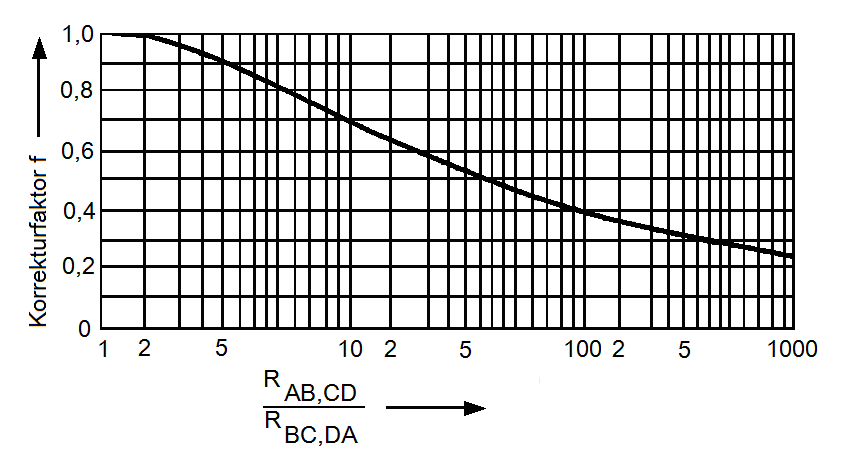
\includegraphics[width=\textwidth]{Figures/Korrekturfaktor.png}
        \caption{Grafik zur Bestimmung des Korrekturfaktors für die
            \textit{van-der-Pauw} Methode.\cite{bib:Anleitung}}
        \label{fig:Korrekturfaktor}
      \end{figure}
      
      Da unsere berechneten Verhältnisse von $R_{12,34}/R_{23,41}$ und
      $R_{34,12}/R_{41,23}$ sehr nahe $1$ sind, nähern wir hier den
      Korrekturfaktor mit $f=1$ an.
      Diese Näherung ist physikalisch erlaubt, da unsere Proben eine ideale,
      symmetrische Geometrie besitzen.
      
      In \cref{tab:SpezifischerWiderstandGaAs,tab:SpezifischerWiderstandInAs}
      sind unsere berechneten Werte für alle fünf Messungen dargestellt.
      \begin{table}[htbp]
        \begin{minipage}{.48\textwidth}
          \centering
          \footnotesize
          \rowcolors{2}{}{lightgray!40}
          \begin{tabular}{ccc}
            $\rho_{1,s}/\SI{}{\ohm\per\meter}$ &
            $\rho_{2,s}/\SI{}{\ohm\per\meter}$ &
            $<\rho_{s}>/\SI{}{\ohm\per\meter}$
            \\ \hline \hline
            9,835 & 9,835 & 9,835 \\
9,835 & 9,835 & 9,835 \\
9,847 & 9,835 & 9,841 \\
9,847 & 9,824 & 9,835 \\
9,824 & 9,824 & 9,824 \\

            \cline{3-3} \cline{3-3}
            & & \SI{9,834(7)}{} \\
          \end{tabular}
          \caption{Spezifische Widerstandswerte für die \textit{GaAs (alt)}
              Probe.}
          \label{tab:SpezifischerWiderstandGaAs}
        \end{minipage}\quad
        \begin{minipage}{.48\textwidth}
          \centering
          \footnotesize
          \rowcolors{2}{}{lightgray!40}
          \begin{tabular}{ccc}
            $\rho_{1,s}/\SI{}{\ohm\per\meter}$ &
            $\rho_{2,s}/\SI{}{\ohm\per\meter}$ &
            $<\rho_{s}>/\SI{}{\ohm\per\meter}$
            \\ \hline \hline
            27,094 & 27,096 & 27,095 \\
27,099 & 27,098 & 27,099 \\
27,099 & 27,099 & 27,099 \\
27,099 & 27,099 & 27,099 \\
27,100 & 27,100 & 27,100 \\

            \cline{3-3} \cline{3-3}
            & & \SI{27,098(2)}{} \\
          \end{tabular}
          \caption{Spezifische Widerstandswerte für die
              \textit{InAs - HF-301-040} Probe.}
          \label{tab:SpezifischerWiderstandInAs}
        \end{minipage}
      \end{table}
      
      Für die tatsächlichen Resultate unserer Messungen bilden wir nun den
      Mittelwert über alle fünf Messungen einer Probe und erhalten damit
      den eigentlichen Wert des spezifischen Widerstandes dieser Probe.
      Die Fehler auf den berechneten Wert gewinnen wir aus der
      Standardabweichung unserer fünf Messungen.
      
      Für die Probe \textit{GaAs (alt)} erhalten wir somit einen Wert von
      $\rho_{s} = \SI{9,834(7)}{\ohm\per\meter}$ für den spezifischen Widerstand.
      Da allerdings nach der elektrischen Leitfähigkeit gefragt ist, erhalten
      wir mit \cref{eq:Leitfähigkeit} die elektrische Leitfähigkeit
      $\sigma_{s} = \SI{1,0169(7)e-1}{\meter\per\ohm}$.
      
      \begin{equation}
        \label{eq:Leitfähigkeit}
        \sigma_{s} = \frac{1}{\rho_{s}}
      \end{equation}
      
      Für die Probe \textit{InAs HF-301-040} erhalten wir
      $\rho_{s} = \SI{27,098(2)}{\ohm\per\meter}$ für den spezifischen
      Widerstand und
      $\sigma_{s} = \SI{3,6903(2)e-2}{\meter\per\ohm}$ für die elektrische
      Leitfähigkeit.
      
    \end{section}
    %%%%%%%%%%%%%%%%%%%%%%%%%%%%%%
   
   
   
    %%%%%%%%%%%%%%%%%%%%%%%%%%%%%%
    %%%%%%%%%%%%%%%%%%%%%%%%%%%%%%
    %%%%%%%%%%%%%%%%%%%%%%%%%%%%%%
    \begin{section}{Hallkonstante bei Raumtemperatur}
      \label{chp:AuswertungHallkonstanteRaumtemperatur}
      Als nächstes können wir aus dem zweiten Satz von Schaltungen
      (\cref{tab:SchalterstellungHall}) die Hallkonstanten beider Proben
      bestimmen.
      
      Bei der Bestimmung der Hallkonstanten gibt es zwei leicht verschiedene
      Möglichkeiten.
      Die Hallkonstante einer Probe kann sowohl aus einer Messung \textbf{mit}
      einer Nullfeldmessung also auch \textbf{ohne} dieses Nullfeld Berechnet
      werden.
      In diesem Experiment führen wir beide Methoden aus um zu überprüfen, ob
      eine Nullfeldmessung tatsächlich notwendig ist.
      
      \begin{subsection}{\textit{Mit} Nullfeldmessung}
        \label{chp:AuswertungHallkonstanteRaumtemperaturMit}
        Zunächst wollen wir die Hallkonstante der beiden Proben mit einer
        Nullfeldmessung berechnen.
        Dazu korrigieren wir die diagonal an der Probe anliegende Spannung mit
        der gemessenen Spannung aus der Nullfeldmessung.
        
        \foureqn{V_{A} = U1-U9  \label{eq:KontaktspannungVA}}
                {V_{B} = U2-U10 \label{eq:KontaktspannungVB}}
                {V_{C} = U5-U9  \label{eq:KontaktspannungVC}}
                {V_{D} = U6-U10 \label{eq:KontaktspannungVD}}
        
        Hierbei ist es nicht notwendig die Spannung über zwei unterschiedlichen
        diagonalen zu messen.
        Wir verwenden daher hier nur die Hallspannungen der Schaltungen
        1, 2, 5 und 6, sowie die Nullfeldschaltungen 9 und 10.
        Die korrigierten Spannungen haben wir in
        \cref{tab:HallKontaktspannungGaAs,tab:HallKontaktspannungInAs} berechnet
        und in \SI{}{\milli\volt} angegeben.
        \begin{table}[htbp]
          \begin{minipage}{.48\textwidth}
            \centering
            \footnotesize
            \rowcolors{2}{}{lightgray!40}
            \begin{tabular}{cccc}
              $V_{A}/mV$ & $V_{B}/mV$ & $V_{C}/mV$ & $V_{D}/mV$ \\ \hline \hline
              0,043 & -0,045 & -0,045 & 0,046 \\
0,043 & -0,044 & -0,046 & 0,045 \\
0,043 & -0,044 & -0,045 & 0,045 \\
0,044 & -0,044 & -0,045 & 0,046 \\
0,043 & -0,045 & -0,045 & 0,044 \\

            \end{tabular}
            \caption{Umgerechnete Kontaktspannungen für die
                \textit{GaAs (alt)} Probe.}
            \label{tab:HallKontaktspannungGaAs}
          \end{minipage}\quad
          \begin{minipage}{.48\textwidth}
            \centering
            \footnotesize
            \rowcolors{2}{}{lightgray!40}
            \begin{tabular}{cccc}
              $V_{A}/mV$ & $V_{B}/mV$ & $V_{C}/mV$ & $V_{D}/mV$ \\ \hline \hline
              26,854 & -26,856 & -26,866 & 26,866 \\
26,846 & -26,847 & -26,869 & 26,870 \\
26,847 & -26,847 & -26,862 & 26,864 \\
26,842 & -26,845 & -26,858 & 26,856 \\
26,830 & -26,830 & -26,849 & 26,850 \\

            \end{tabular}
            \caption{Umgerechnete Kontaktspannungen für die 
                \textit{InAs - HF-301-040} Probe.}
            \label{tab:HallKontaktspannungInAs}
          \end{minipage}
        \end{table}
        
        Aus den korrigierten Kontaktspannungen kann nun die Hallspannung
        berechnet werden.
        Dazu bilden wir den Mittelwert, z.B. der beiden Kontaktspannungen
        $V_{A}$ und $V_{B}$ die Spannung an den selben Punkten abgreift, der
        Strom aber in entgegengesetzte Richtung fließt.
        Um die Hallspannungen zu berechnen benutzen wir daher
        \cref{eq:HallspannungPos,eq:HallspannungNeg}
        
        \twoeqn{V_{H+} = \frac{V_{A}-V_{B}}{2} \label{eq:HallspannungPos}}
               {V_{H-} = -\frac{V_{C}-V_{D}}{2}. \label{eq:HallspannungNeg}}
        
        Aus den damit bestimmten Hallspannungen für beide Proben, lassen sich
        nun ihre die Hallkonstanten errechnen.
        Dazu verwenden wir die
        \cref{eq:HallKonstantemitPos,eq:HallKonstantemitNeg}
        
        \twoeqn{R_{H+} = \frac{V_{H+}}{IB_{+}} \label{eq:HallKonstantemitPos}}
               {R_{H-} = \frac{V_{H-}}{IB_{-}}.\label{eq:HallKonstantemitNeg}}
        
        Dargestellt sind die Werte nun in den
        \cref{tab:HallKonstanteGaAsmit,tab:HallKonstanteInAsmit}.
        
        \begin{table}[htbp]
          \centering
          \footnotesize
          \rowcolors{2}{}{lightgray!40}
          \begin{tabular}{cccc}
            $V_{H+}/mV$ & $V_{H-}/mV$ &
            $R_{H+}/\SI{}{\meter\squared\per\coulomb}$ &
            $R_{H-}/\SI{}{\meter\squared\per\coulomb}$ \\ \hline \hline
            0,044 & 0,046 & 3,188 & 3,297 \\
0,044 & 0,046 & 3,152 & 3,297 \\
0,044 & 0,045 & 3,152 & 3,261 \\
0,044 & 0,046 & 3,188 & 3,297 \\
0,044 & 0,045 & 3,188 & 3,225 \\

            \hiderowcolors
            \cline{3-4} \cline{3-4}
            & & \multicolumn{2}{c}{\SI{3,225(23)}{}} \\
          \end{tabular}
          \caption{Hallspannungen und Hallkonstanten für die
              \textit{GaAs (alt)} Probe.}
          \label{tab:HallKonstanteGaAsmit}
        \end{table}
        
        \begin{table}[htbp]
          \centering
          \footnotesize
          \rowcolors{2}{}{lightgray!40}
          \begin{tabular}{cccc}
            $V_{H+}/mV$ & $V_{H-}/mV$ &
            $R_{H+}/\SI{}{\meter\squared\per\coulomb}$ &
            $R_{H-}/\SI{}{\meter\squared\per\coulomb}$ \\ \hline \hline
            26,855 & 26,866 & 12,971 & 12,976 \\
26,847 & 26,870 & 12,967 & 12,978 \\
26,847 & 26,863 & 12,967 & 12,975 \\
26,844 & 26,857 & 12,965 & 12,972 \\
26,830 & 26,850 & 12,959 & 12,968 \\

            \hiderowcolors
            \cline{3-4} \cline{3-4}
            & & \multicolumn{2}{c}{\SI{12,9697(37)}{}} \\
          \end{tabular}
          \caption{Hallspannungen und Hallkonstanten für die 
              \textit{InAs - HF-301-040} Probe.}
          \label{tab:HallKonstanteInAsmit}
        \end{table}
        
        Für die Messung der Hallkonstanten mithilfe der Nullfeldmessung ergibt
        sich also für die \textit{GaAs (alt)} Probe ein Mittelwert von
        $R_{H} = \SI{3,225(23)}{\meter\squared\per\coulomb}$.
        Für die \textit{InAs-HF-301-040} ergibt sich eine mittlere Hallkonstante
        von $R_{H} = \SI{12,9697(37)}{\meter\squared\per\coulomb}$.
        Die Fehler ergeben sich hierbei aus den Standardabweichungen der fünf
        Messungen.
        
      \end{subsection}
      
      
      
      \begin{subsection}{\textit{Ohne} Nullfeldmessung}
        \label{chp:AuswertungHallkonstanteRaumtemperaturOhne}
        Die Hallkonstante einer Probe lässt sich aber auch ohne eine
        Nullfeldmessung bestimmen.
        Anders als bei der Nullfeldmessung werden die Kontaktspannungen hier
        nicht gegen ein Nullfeld korrigiert sondern direkt in die Gleichung
        der Hallkonstanten eingebracht.
        Zunächst wird der Mittelwert der Kontaktspannungen gleicher Anschlüsse
        bestimmt
        (\crefrange{eq:KontaktspannungVAohne}{eq:KontaktspannungVDohne}).
        
        \foureqn{V_{A} = \frac{U1-U2}{2} \label{eq:KontaktspannungVAohne}}
                {V_{B} = \frac{U3-U4}{2} \label{eq:KontaktspannungVBohne}}
                {V_{C} = \frac{U5-U6}{2} \label{eq:KontaktspannungVCohne}}
                {V_{D} = \frac{U7-U8}{2} \label{eq:KontaktspannungVDohne}}
        
        Anschließend bilden wir den Mittelwert über die Spannungen beider
        magnetischen Polarisationen
        (\cref{eq:Hallspannung1,eq:Hallspannung2}).
        
        \twoeqn{V_{H1,S} = \frac{V_{A}-V_{C}}{2} \label{eq:Hallspannung1}}
               {V_{H2,S} = \frac{V_{B}-V_{D}}{2} \label{eq:Hallspannung2}}
        
        Ab hier berechnet sich die Hallkonstante ähnlich der
        \textbf{mit Nullfeld} Methode.
        Die über \cref{eq:Hallkonstanteohne1,eq:Hallkonstanteohne2} berechneten
        Hallkonstanten 
        
        \twoeqn{R_{H1,S} = \frac{V_{H1,S}}{IB_{+}} \label{eq:Hallkonstanteohne1}}
               {R_{H2,S} = \frac{V_{H2,S}}{IB_{-}} \label{eq:Hallkonstanteohne2}}
        
        sind in \cref{tab:HallKonstanteGaAsohne,tab:HallKonstanteInAsohne}
        dargestellt.
        
        \begin{table}[htbp]
          \begin{minipage}{.48\textwidth}
            \centering
            \footnotesize
            \rowcolors{2}{}{lightgray!40}
            \begin{tabular}{ccc}
              $R_{H+}/\SI{}{\meter\squared\per\coulomb}$ &
              $R_{H-}/\SI{}{\meter\squared\per\coulomb}$ &
              $R_{H}/\SI{}{\meter\squared\per\coulomb}$ \\ \hline \hline
              3,243 & 3,225 & 3,234 \\
3,225 & 3,207 & 3,216 \\
3,207 & 3,216 & 3,211 \\
3,243 & 3,225 & 3,234 \\
3,207 & 3,225 & 3,216 \\

              \hiderowcolors
              \cline{3-3}
              & & \SI{3,222(12)}{} \\
            \end{tabular}
            \caption{Hallkonstanten für die \textit{GaAs (alt)} Probe.}
            \label{tab:HallKonstanteGaAsohne}
          \end{minipage}\quad
          \begin{minipage}{.48\textwidth}
            \centering
            \footnotesize
            \rowcolors{2}{}{lightgray!40}
            \begin{tabular}{ccc}
              $R_{H+}/\SI{}{\meter\squared\per\coulomb}$ &
              $R_{H-}/\SI{}{\meter\squared\per\coulomb}$ &
              $R_{H}/\SI{}{\meter\squared\per\coulomb}$ \\ \hline \hline
              12,973 & 12,967 & 12,970 \\
12,972 & 12,966 & 12,969 \\
12,971 & 12,964 & 12,968 \\
12,969 & 12,962 & 12,965 \\
12,963 & 12,958 & 12,961 \\

              \hiderowcolors
              \cline{3-3}
              & & \SI{12,9666(34)}{} \\
            \end{tabular}
            \caption{Hallkonstanten für die \textit{InAs - HF-301-040} Probe.}
            \label{tab:HallKonstanteInAsohne}
          \end{minipage}
        \end{table}
        
        Für die Messung der Hallkonstanten ohne die Nullfeldmessung ergibt
        sich also für die \textit{GaAs (alt)} Probe ein Mittelwert von
        $R_{H} = \SI{3,222(12)}{\meter\squared\per\coulomb}$.
        Für die \textit{InAs-HF-301-040} ergibt sich eine mittlere Hallkonstante
        von $R_{H} = \SI{12,9666(34)}{\meter\squared\per\coulomb}$.
        Die Fehler ergeben sich hierbei aus den Standardabweichungen der fünf
        Messungen.
        
      \end{subsection}
      
      Aus den Resultaten der beiden Methoden ist mit
      $R_{H} = \SI{3,225(23)}{\meter\squared\per\coulomb}$ und
      $R_{H} = \SI{3,222(12)}{\meter\squared\per\coulomb}$ für die
      \textit{GaAs (alt)} Probe, sowie
      $R_{H} = \SI{12,9697(37)}{\meter\squared\per\coulomb}$ und
      $R_{H} = \SI{12,9666(34)}{\meter\squared\per\coulomb}$ für die
      \textit{InAs-HF-301-040} Probe schnell ersichtlich, dass beide Methoden
      im selben Fehlerbereich liegen und es somit keine Auswirkungen hat welche
      der Methoden tatsächlich verwendet wird.
      
    \end{section}
    %%%%%%%%%%%%%%%%%%%%%%%%%%%%%%
    
    
    
    %%%%%%%%%%%%%%%%%%%%%%%%%%%%%%
    %%%%%%%%%%%%%%%%%%%%%%%%%%%%%%
    %%%%%%%%%%%%%%%%%%%%%%%%%%%%%%
    \begin{section}{Beweglichkeit der Ladungen}
      \label{chp:AuswertungBeweglichkeitLadungen}
      Nachdem nun alle Grundlegenden Größen der Proben bestimmt wurden, sollen
      nun auch noch die Beweglichkeit $\mu_{S}$ und die Ladungsträgerdichte der
      Majoritätsladungen $p_{S}$ bestimmt werden.
      
      Dazu verwenden wir die \cref{eq:Beweglichkeit,eq:Ladungstraegerdichte}
      
      \twoeqn{\mu_{S} = \left| \frac{R_{H,S}}{\rho_{S}} \right|
                \label{eq:Beweglichkeit}}
             {p_{S} = \frac{1}{e\cdot R_{H,S}}. \label{eq:Ladungstraegerdichte}}
      
      Die resultierenden Werte sind in
      \cref{tab:BeweglichkeitLadungstraegerdichte} notiert.
      
      \begin{table}[htbp]
        \centering
        \begin{tabular}{c|c|c}
          Probe & $\mu_{H,S}/\SI{}{\meter\squared\per\volt\per\second}$ &
          $p_{H,S}/\SI{}{\meter\squared}$ \\ \hline
          \textit{GaAs (alt)} & \SI{3,276(10)e-1}{} & \SI{1,937(6)e+18}{} \\
%           \hline
          \textit{InAs-HF-301-040} & \SI{4,785(1)e-1}{} & \SI{4,814(1)e+17}{} \\
        \end{tabular}
        \caption{Berechnete Werte der Beweglichkeit und Ladungsträgerdichte
            der Majoritätsladungen.}
        \label{tab:BeweglichkeitLadungstraegerdichte}
      \end{table}
      
      \todo{Fertig? oder kann man noch mehr sagen?}
      
    \end{section}
    %%%%%%%%%%%%%%%%%%%%%%%%%%%%%%
   
   
   
    %%%%%%%%%%%%%%%%%%%%%%%%%%%%%%
    %%%%%%%%%%%%%%%%%%%%%%%%%%%%%%
    %%%%%%%%%%%%%%%%%%%%%%%%%%%%%%
    \begin{section}{Temperaturabhängigkeit}
      \label{chp:AuswertungTemperaturen}
      Der zweite Teil dieses Experimentes besteht darin, dass wir die zuvor
      bei Raumtemperatur bestimmten physikalischen Größen nun bei einer Probe
      auf eine Temperaturabhängigkeit untersuchen wollen.
      Wir haben dazu die \textit{InAs-HF-301-040} Probe ausgewählt.
      Anders als im ersten Versuchsteil nehmen wir nun allerdings nicht mehr
      fünf Messwerte für jede Messung, sondern beschränken uns hier auf einzelne
      Messwerte.
      
      Alle zuvor beschriebenen Berechnungen werden nun auf die Messwerte aus
      \cref{tab:TemperaturInAs} angewandt.
      Die damit bestimmten Werte werden hier in
      \cref{tab:TemperaturInAsResultate} dargestellt.
      
      \begin{table}[htbp]
        \centering
        \footnotesize
        \rowcolors{2}{}{lightgray!40}
        \begin{tabular}{c|c|c|c|c|c}
          T/\SI{}{\celsius} & $T_{inv}/\SI{}{\per\kelvin}$ &
          $\sigma_{S}/\SI{}{\meter\per\ohm}$ &
          $R_{H,S}/\SI{}{\meter\squared\per\coulomb}$ &
          $p_{H,S}/\SI{}{\meter\squared}$ &
          $\mu_{H,S}/\SI{}{\meter\squared\per\volt\per\second}$ \\ \hline
          -205,5 & 0,0148 & 0,0402 & 13,254 & 4,710E+17 & 0,533 \\
-195,5 & 0,0129 & 0,0402 & 13,273 & 4,703E+17 & 0,533 \\
-183 & 0,0111 & 0,0400 & 13,279 & 4,701E+17 & 0,531 \\
-172,5 & 0,0099 & 0,0398 & 13,280 & 4,700E+17 & 0,529 \\
-161,5 & 0,0090 & 0,0397 & 13,272 & 4,703E+17 & 0,526 \\
-152 & 0,0083 & 0,0395 & 13,272 & 4,703E+17 & 0,525 \\
-140 & 0,0075 & 0,0395 & 13,259 & 4,708E+17 & 0,523 \\
-125 & 0,0067 & 0,0392 & 13,238 & 4,715E+17 & 0,519 \\
-109,5 & 0,0061 & 0,0389 & 13,203 & 4,728E+17 & 0,514 \\
-93 & 0,0056 & 0,0387 & 13,178 & 4,737E+17 & 0,510 \\
-79 & 0,0052 & 0,0384 & 13,152 & 4,746E+17 & 0,505 \\
-63 & 0,0048 & 0,0380 & 13,122 & 4,757E+17 & 0,499 \\
-27 & 0,0041 & 0,0373 & 13,031 & 4,790E+17 & 0,486 \\
0 & 0,0037 & 0,0368 & 12,956 & 4,818E+17 & 0,477 \\

        \end{tabular}
        \caption{Berechnete physikalische Messgrößen für verschiedene
            Temperaturen.}
        \label{tab:TemperaturInAsResultate}
      \end{table}
      
      In den \crefrange{fig:TempLeifaehigkeit}{fig:TempLadungsdichte} haben
      wir die bestimmten Größen gegen die inverse Temperatur aufgetragen.
      
      \begin{figure}[ht!]
        \centering
        \begin{minipage}{.92\textwidth}
          \centering
          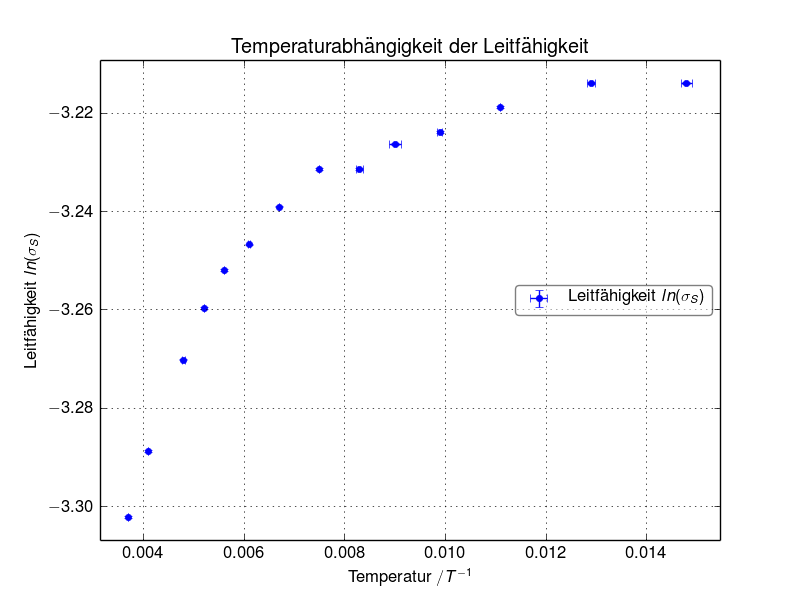
\includegraphics[width=\textwidth]{Figures/Temp_Leitfaehigkeit.png}
          \caption{Leitfähigkeit gegen invertierte Temperatur
              \SI{}{\per\kelvin}.}
          \label{fig:TempLeifaehigkeit}
        \end{minipage}\\
        \begin{minipage}{.92\textwidth}
          \centering
          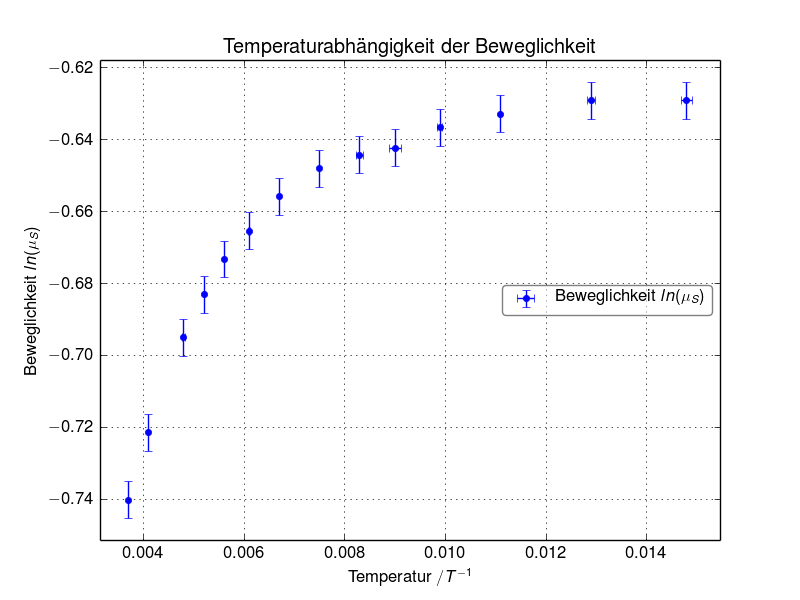
\includegraphics[width=\textwidth]{Figures/Temp_Beweglichkeit.png}
          \caption{Beweglichkeit gegen invertierte Temperatur
              \SI{}{\per\kelvin}.}
          \label{fig:TempBeweglichkeit}
        \end{minipage}
      \end{figure}
      
      \newpage
      \begin{figure}[ht!]
        \centering
        \begin{minipage}{.92\textwidth}
          \centering
          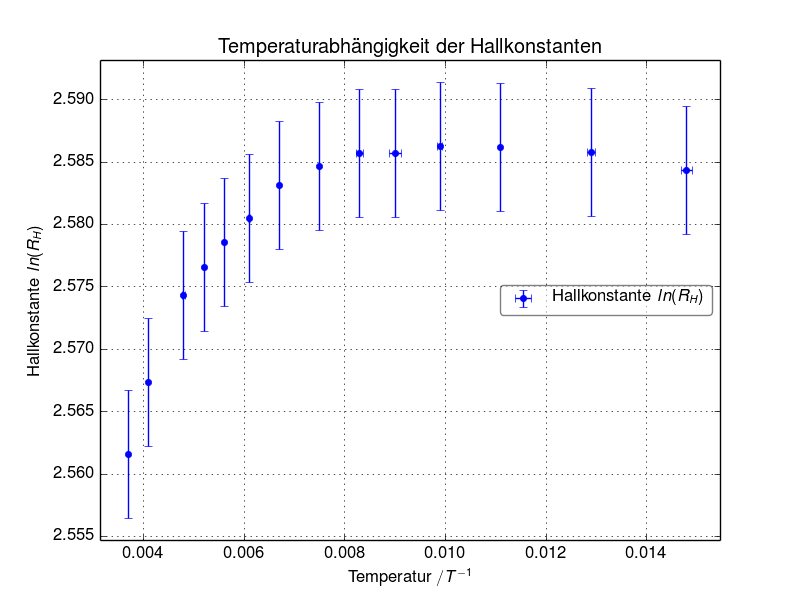
\includegraphics[width=\textwidth]{Figures/Temp_Hallkonstante.png}
          \caption{Hallkonstante gegen invertierte Temperatur
              \SI{}{\per\kelvin}.}
          \label{fig:TempHallkonstante}
        \end{minipage}\\
        \begin{minipage}{.92\textwidth}
          \centering
          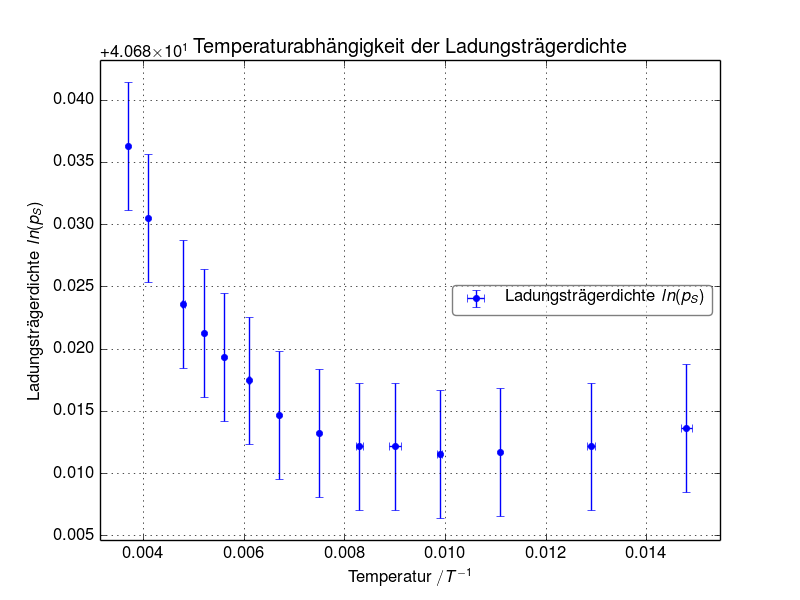
\includegraphics[width=\textwidth]{Figures/Temp_Ladungsdichte.png}
          \caption{Ladungsträgerdichte der Majoritätsladungen gegen invertierte
              Temperatur \SI{}{\per\kelvin}.}
          \label{fig:TempLadungsdichte}
        \end{minipage}
      \end{figure}
      
      
    \end{section}
    %%%%%%%%%%%%%%%%%%%%%%%%%%%%%%
    
    
    
    \newpage
    %%%%%%%%%%%%%%%%%%%%%%%%%%%%%%
    %%%%%%%%%%%%%%%%%%%%%%%%%%%%%%
    %%%%%%%%%%%%%%%%%%%%%%%%%%%%%%
    \begin{section}{Fazit}
      \label{chp:Fazit}
      
      
      
    \end{section}
    %%%%%%%%%%%%%%%%%%%%%%%%%%%%%%
    
  \end{chapter}
  %%%%%%%%%%%%%%%%%%%%
  
  
  
  %%%%%%%%%%%%%%%%%%%%
  %%%%%%%%%%%%%%%%%%%%
  %%%%%%%%%%%%%%%%%%%%
  %%%%%%%%%%%%%%%%%%%%
%%%%%%%%%%%%%%%%%%%%
%%%%%%%%%%%%%%%%%%%%
\begin{appendix}
  \label{Anhang}
  
  
  
  %%%%%%%%%%%%%%%%%%%%%%%%%%%%%%
  %%%%%%%%%%%%%%%%%%%%%%%%%%%%%%
  %%%%%%%%%%%%%%%%%%%%%%%%%%%%%%
  \begin{chapter}{ERSTER TEIL}
    \label{Anhang:chp:ERSTERTEIL}
    
    
    
  \end{chapter}
  %%%%%%%%%%%%%%%%%%%%%%%%%%%%%%
  
  
  
  %%%%%%%%%%%%%%%%%%%%%%%%%%%%%%
  %%%%%%%%%%%%%%%%%%%%%%%%%%%%%%
  %%%%%%%%%%%%%%%%%%%%%%%%%%%%%%
  \begin{chapter}{ZWEITER TEIL}
    \label{Anhang:chp:ZWEITERTEIL}
    
    
    
  \end{chapter}
  %%%%%%%%%%%%%%%%%%%%%%%%%%%%%%
  
\end{appendix}
%%%%%%%%%%%%%%%%%%%%
 
  %%%%%%%%%%%%%%%%%%%%
  
  
  
  %%%%%%%%%%%%%%%%%%%%
  %%%%%%%%%%%%%%%%%%%%
  %%%%%%%%%%%%%%%%%%%%
  \begin{thebibliography}{99}
    \scriptsize
    \bibitem{bib:Anleitung}\url{http://www.praktika.physik.uni-bonn.de/module/physik412/downloads/p441d}
\bibitem{bib:}\url{bla}
  \end{thebibliography}
  %%%%%%%%%%%%%%%%%%%%
 
\end{document}
%%%%%%%%%%
